\begin{frame}
  \HUGE
  BACKUP
\end{frame}

\begin{frame}\frametitle{Parton Distribution Functions}
  \begin{figure}[htb]
    \begin{center}
       \includegraphics[width=0.80\textwidth]{../figs/Intro/pdfs.png} 
    \end{center}
  \end{figure}
\end{frame}%{WGamma, LO and NLO Feynman diagrams}

\begin{frame}\frametitle{WGamma, LO and NLO Feynman diagrams}
  \begin{figure}[htb]
    \begin{center}
       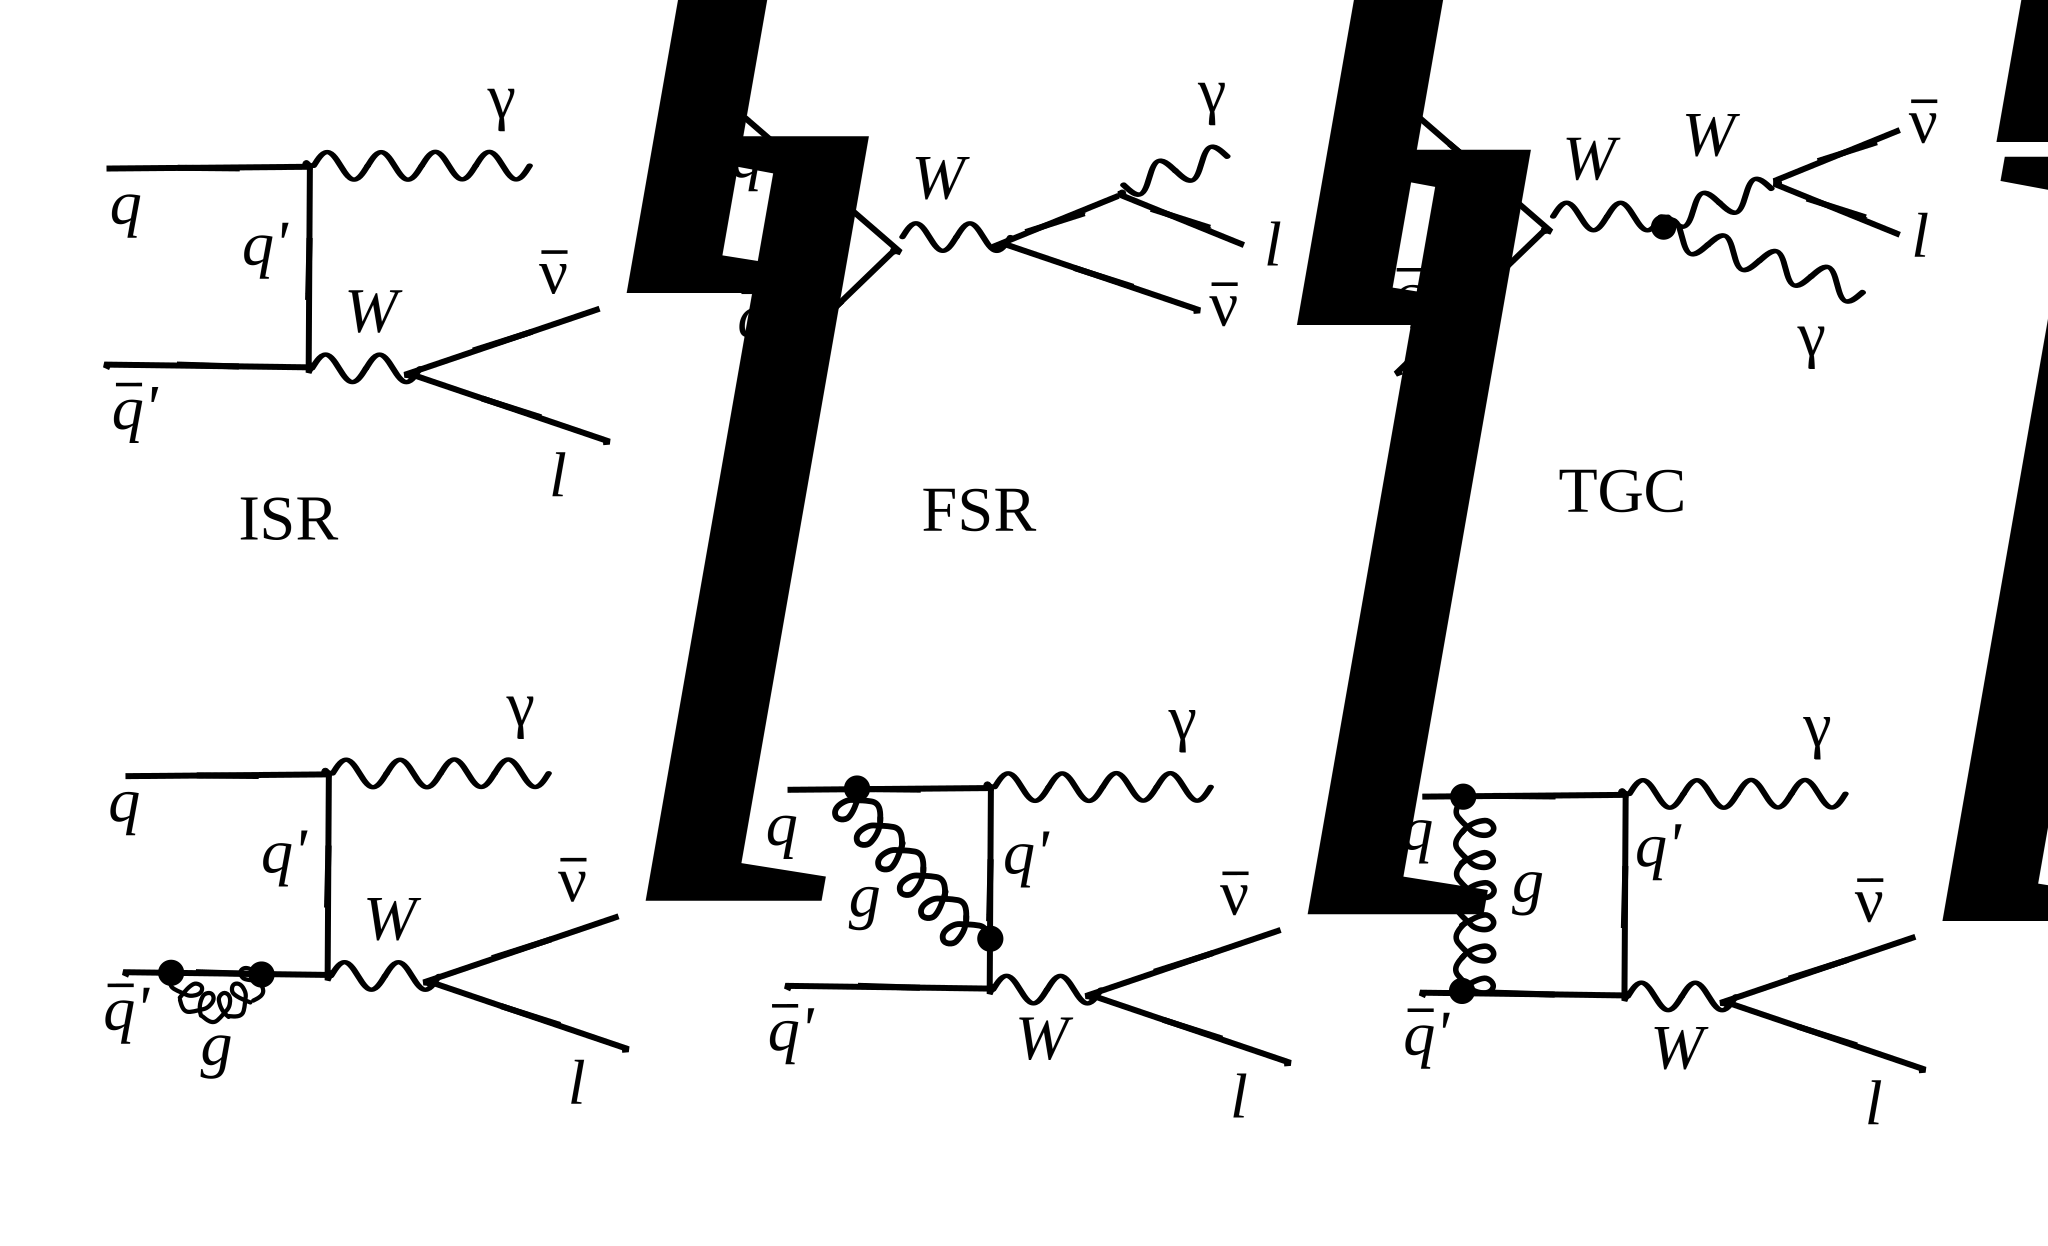
\includegraphics[width=0.85\textwidth]{../figs/WgAbout/feynmWg_LO_NLO.png} 
    \end{center}
  \end{figure}
\end{frame}%{WGamma, LO and NLO Feynman diagrams}

\begin{frame}\frametitle{Data and Simulation Samples}
\scriptsize
Data: CMS experiment, 2012,  $pp$ collisions at $\sqrt{s}=$8~TeV\\
Integrated luminosity: $L=$19.6~fb$^{-1}$ 

\begin{table}[h]
  \scriptsize
  \begin{center}
    \begin{tabular}{|l|l|l|l|}
      \hline
      Dataset          & Candidates                        &  Purpose   & Size, T   \\ \hline
      Single muon      & $W\gamma\rightarrow\mu\nu\gamma$  &  target process   & 1.2 \\ \hline %(NLO MCFM)
      Single electron  & $W\gamma\rightarrow e\nu\gamma$   &  target process   & 2.0 \\ \hline %(NNLO FEWZ)
      Double muon      & $Z\gamma\rightarrow\mu\mu\gamma$  &  background estimation   & 0.4 \\ \hline %(NNLO FEWZ)
      Double electron  & $Z\gamma\rightarrow ee\gamma$     &  background estimation   & 0.5 \\ \hline %(NNLO)
    \end{tabular}
  \end{center}
\end{table} 

\scriptsize
Monte Carlo Simulation (MC) samples:\\

\begin{table}[h]
  \scriptsize
  \begin{center}
 %   \caption{Summary of simulated samples used in the measurement.}
    \begin{tabular}{|l|l|l|}
      \hline
      Process                              & Type & $\sigma$, pb  \\ \hline
      $W\gamma \rightarrow l\nu\gamma$     & signal & 554   \\ \hline %(NLO MCFM)
      $W$+jets$ \rightarrow l\nu $+jets   & background & 36257  \\ \hline %(NNLO FEWZ)
      DY+jets$ \rightarrow ll $+jets     & background & 3504  \\ \hline %(NNLO FEWZ)
      $t\bar{t}$+jets$\rightarrow 1l$+X    & background & 99    \\ \hline %(NNLO)
      $t\bar{t}$+jets$\rightarrow 2l$+X    & background & 24    \\ \hline
      $Z\gamma \rightarrow ll\gamma$       & background & 172   \\ \hline
    \end{tabular}
    \label{tab:mc_bkg_samples}
  \end{center}
\end{table} 

\end{frame}%{MC Samples and Luminosity Reweighting}

\begin{frame}\frametitle{Comment about PU from Wgg CMS Analysis Note}
  \begin{figure}[htb]
    \begin{center}
       \includegraphics[width=0.65\textwidth]{../figs/ForPresentation/PUmultiplicityCorrection_Wgg.png} 
    \end{center}
  \end{figure}
\end{frame}%{Comment about PU from Wgg note}

\begin{frame}\frametitle{$P_T^{\gamma}$ Spectrum of $W\gamma$ Candidates, Two Channels}
  \begin{figure}[htb]
    \begin{center}
       \includegraphics[width=0.49\textwidth]{../figs/figs_v11/MUON_WGamma/PrepareYields/c_TotalDATAvsMC_Barrel__phoEt.pdf} \includegraphics[width=0.49\textwidth]{../figs/figs_v11/ELECTRON_WGamma/PrepareYields/c_TotalDATAvsMC_Barrel__phoEt.pdf} 
    \end{center}
  \end{figure}

\tiny
  \begin{table}[h]
     \tiny
     \begin{center}
     \begin{tabular}{|l|l|}
     \hline
     {\bfseries{Comments:}} &  {\bfseries{ Backgrounds:}}\\ 
     Dominated by $W$+jets events in low $P_T^{\gamma}$ bins; & Jets$\rightarrow\gamma$: $W$+jets, DY+jets, $t\bar{t}$+jets;\\
     Fraction of signal increases with $P_T^{\gamma}$; & $e\rightarrow\gamma$: DY+jets (electron channel only);\\
     Data disagree with MC.          & Real-$\gamma$: $Z\gamma$, $W\gamma\rightarrow\tau\nu\gamma$.\\
     \hline
      \end{tabular}
      \end{center}
  \end{table}

\end{frame}

\begin{frame}\frametitle {$e\rightarrow\gamma$ and Real-$\gamma$ Backgrounds}

  \begin{table}[h]
     \tiny
     \begin{center}
     \begin{tabular}{|l|l|l|l|}
     \hline
     Type & Source & Comment & Estimation \\ \hline
     $e\rightarrow\gamma$ & DY+jets$\rightarrow ee$+jets & no track for $e$; fake $E_T^{miss}$ & semi data driven\\\hline
     Real-$\gamma$ & $Z\gamma \rightarrow ll\gamma$ & pass second lepton veto; fake $E_T^{miss}$ & MC-based\\\hline
     Real-$\gamma$ & $W\gamma \rightarrow \tau\nu\gamma$ & $\tau^- \rightarrow \mu^- \bar{\nu_{\mu}} \nu_{\tau}$ and $\tau^- \rightarrow e^- \bar{\nu_{e}} \nu_{\tau}$ & MC-based\\
     \hline
      \end{tabular}
      \end{center}
  \end{table}

\begin{figure}[htb]
  \begin{center}
   \includegraphics[width=0.32\textwidth]{../figs/figs_v11/MUON_WGamma/PrepareYields/c_TotalDATAvsMC_EtaCommon__WMtVERY_PRELIMINARY.pdf}\includegraphics[width=0.32\textwidth]{../figs/figs_v11/ELECTRON_WGamma/PrepareYields/c_TotalDATAvsMC_EtaCommon__WMtVERY_PRELIMINARY.pdf}\includegraphics[width=0.32\textwidth]{../figs/figs_v11/ELECTRON_WGamma/PrepareYields/c_TotalDATAvsMC_EtaCommon__Mpholep1PRELIMINARY_FOR_E_TO_GAMMA_WITH_PSV_CUT.pdf}
  \end{center}
\end{figure}
\tiny
$M_T^W>40$~GeV in both channels: rejects events without $E_T^{miss}$\\
$M_{l,\gamma}<70~or~M_{l,\gamma}>110$~GeV in the electron channel: rejects events from DY+jets$\rightarrow ee$+jets \\
{\bfseries{Non-negligible amount remains}}\\
\begin{itemize}
  \item Invariant mass of a particle system ($M_{ab} = m_a^2+m_b^2+2(E_aE_b-{\bfseries{p_a\cdot p_b}})$)
  \item Transverse mass of a $W$ boson ($M_T^W=\sqrt{2  P_T^{l}  E_T^{miss}  (1-\cos{(\phi^{l}-\phi^{miss})})}$)
\end{itemize}

\end{frame}%{$e\rightarrow\gamma$ and Real-$\gamma$ Backgrounds}

\begin{frame}\frametitle{\footnotesize{$P_T^{\gamma}$ Spectrum (ECal Barrel Only). Both channels}}
   \begin{figure}[htb]
    \begin{center}
       \includegraphics[width=0.30\textwidth]{../figs/figs_v11/MUON_WGamma/PrepareYields/c_DATAvsBkgPlusSigMCc_MUON_WGamma_TEMPL_CHISO_UNblind__Barrel__phoEt.pdf}\includegraphics[width=0.30\textwidth]{../figs/figs_v11/MUON_WGamma/PrepareYields/c_DATAvsBkgPlusSigMCc_MUON_WGamma_TEMPL_SIHIH_UNblind__Barrel__phoEt.pdf}\includegraphics[width=0.30\textwidth]{../figs/figs_v11/MUON_WGamma/PrepareYields/c_BkgSubtrDATAvsSIGMC_c_MUON_WGamma__UNblind__Barrel__phoEt.pdf}\\
       \includegraphics[width=0.30\textwidth]{../figs/figs_v11/ELECTRON_WGamma/PrepareYields/c_DATAvsBkgPlusSigMCc_ELECTRON_WGamma_TEMPL_CHISO_UNblind__Barrel__phoEt.pdf}\includegraphics[width=0.30\textwidth]{../figs/figs_v11/ELECTRON_WGamma/PrepareYields/c_DATAvsBkgPlusSigMCc_ELECTRON_WGamma_TEMPL_SIHIH_UNblind__Barrel__phoEt.pdf}\includegraphics[width=0.30\textwidth]{../figs/figs_v11/ELECTRON_WGamma/PrepareYields/c_BkgSubtrDATAvsSIGMC_c_ELECTRON_WGamma__UNblind__Barrel__phoEt.pdf}\\
    \end{center}
  \end{figure}
\end{frame}%{$jets \rightarrow \gamma$ Background Subtraction. Plots, W$\gamma$}

\begin{frame}\frametitle{Other Corrections}

\begin{table}[h]
  \tiny
  \begin{center}
  \begin{tabular}{|l|c|c|}
    \hline
          & \multicolumn{2}{|c|}{Algebraic representation for} \\ 
     Step & \multicolumn{2}{|c|}{the measurement of} \\ 
          & $d\sigma/dP_{T}^{\gamma}$ & $\sigma$ \\ \hline
    select events & {\bfseries{$N_{sel}^j$}} &    {\bfseries{$N_{sel}$}}       \\ \hline
    subtract background & {\bfseries{$N_{sign}^j = N_{sel}^j - N_{bkg}^j$}} &    {\bfseries{$N_{sign}=N_{sel}-N_{bkg}$}}       \\ \hline
    \multicolumn{3}{|c|}{ } \\  
    \multicolumn{3}{|c|}{NEXT MEASUREMENT STEPS:} \\  
    \multicolumn{3}{|c|}{ } \\ \hline 
    {\bfseries\color{blue}{unfold}}   & {\color{blue}$N_{A\times\epsilon}^i = U_{ij} \cdot N_{sign}^j$} &    $-$       \\ \hline
    {\bfseries\color{blue}{correct for eff X acc}} & {\color{blue}$N_{true}^i = \frac{N_{A\times\epsilon}^i}{(A \times\epsilon)^i}$} &  {\color{blue}$N_{true}=\frac{N_{sign}}{A\times\epsilon}$}       \\ \hline
    compute cross section & $ \left( \frac{d\sigma}{dP_{T}^\gamma} \right) ^i = \frac{N_{true}^i}{L \cdot (\Delta P_T^\gamma)^i}$  &  $\sigma = N_{true}/L$       \\ \hline
    \multicolumn{3}{|l|}{estimate systematic uncertainties }         \\ \hline
  \end{tabular}
  \label{tab:analysisOutline}
  \end{center}
\end{table}

\scriptsize
{\bfseries{Detector resolution unfolding}} (step {\bfseries\color{blue}{``unfold''}}): 
  \begin{itemize} 
    \tiny
    \item {\bfseries{Effect:}} bin-to-bin migration during the $P_T^{\gamma}$ reconstruction; 
    \item {\bfseries{Method:}} D'Agostini, signal MC sample is used;
    \item {\bfseries{Note:}} uncertainties across difffent $P_T^{\gamma}$ bins become correlated.
  \end{itemize}

{\bfseries{Efficiency and Acceptance}} (step {\bfseries\color{blue}{``correct for eff X acc''}}): 
  \begin{itemize} 
    \tiny
    \item {\bfseries{Effect (main):}} lose signal events due to selection criteria applied;
    \item {\bfseries{Method:}} bin-by-bin correction by $A\times\epsilon$, constants prepared using signal MC sample;
    \item {\bfseries{Note:}} efficiencies between data and MC differ (next slide).
  \end{itemize}

\end{frame}%{Other Corrections}

\begin{frame}\frametitle{Efficiency Scale Factors}

\tiny
The scale factors (SF) $\rho = \frac{\epsilon_{data}}{\epsilon_{MC}}$. SF are applied as weights on each event in each MC sample.

\begin{table}[h]
  \tiny
  \begin{center}
   \begin{tabular}{|c|c|}
\hline
 type of candidate                  &   full event SF\\ 
 $W\gamma\rightarrow\mu\nu\gamma$   &   $\rho^{\mu}_{ID\_iso} \times \rho^{\gamma}_{ID}$    \\
 $W\gamma\rightarrow e\nu\gamma$    &   $\rho^{e}_{ID} \times \rho^{\gamma}_{ID}\times \rho^{\gamma}_{PSV}$       \\ \hline
  \end{tabular}
  \label{tab:SFs_Applied}
  \end{center}
\end{table}
Provided by POG: $\rho^{\mu}_{ID\_iso}$, $\rho^{\gamma}_{ID}$,  $\rho^{e}_{ID}$;       provided by $W\gamma\gamma$ measurement: $\rho^{\gamma}_{PSV}$

{\begin{center}$\rho^{\gamma}_{ID}$: \end{center}}
\begin{table}[h]
  \tiny
  \begin{center}
   \begin{tabular}{|c|c|c|c|c|}
\hline
 $P_T^{\gamma}$  & $|\eta^{\gamma}|\leq 0.80$ & $0.80<|\eta^{\gamma}|\leq 1.44$ & $1.57<|\eta^{\gamma}|\leq 2.00$ & $|\eta^{\gamma}|> 2.00$\\ \hline
15-20          & 0.95$\pm$0.02   & 0.99$\pm$0.02        & 1.00$\pm$0.02        & 1.02$\pm$0.02 \\ \hline
20-30          & 0.96$\pm$0.01   & 0.97$\pm$0.01        & 0.98$\pm$0.01        & 1.00$\pm$0.01 \\ \hline
30-40          & 0.98$\pm$0.01   & 0.98$\pm$0.01        & 0.99$\pm$0.01        & 1.00$\pm$0.01 \\ \hline
40-50          & 0.98$\pm$0.01   & 0.98$\pm$0.01        & 1.00$\pm$0.01        & 1.01$\pm$0.01 \\ \hline
$>$50          & 0.98$\pm$0.01   & 0.98$\pm$0.01        & 1.00$\pm$0.01        & 1.01$\pm$0.01 \\ \hline
  \end{tabular}
  \label{tab:SFs_PhotonID}
  \end{center}
\end{table}

{\begin{center}$\rho^{\gamma}_{PSV}$: \end{center}}
\begin{table}[h]
  \tiny
  \begin{center}
   \begin{tabular}{|c|c|c|}
\hline
 $P_T^{\gamma}$  & barrel              & endcap \\ \hline
15-20          & 0.996$\pm$0.020     & 0.960$\pm$0.041 \\ \hline
20-25          & 0.994$\pm$0.024     & 0.977$\pm$0.051 \\ \hline
25-30          & 0.996$\pm$0.030     & 0.951$\pm$0.062 \\ \hline
30-40          & 0.999$\pm$0.033     & 1.029$\pm$0.081 \\ \hline
40-50          & 1.009$\pm$0.073     & {\bfseries\color{blue}{0.971$\pm$0.150}} \\ \hline
50-70          & {\bfseries\color{blue}{0.993$\pm$0.128}}     & {\bfseries\color{blue}{0.965$\pm$0.294}} \\ \hline
$>$70          & {\bfseries\color{blue}{1.047$\pm$0.111}}     & {\bfseries\color{blue}{1.145$\pm$0.371}} \\ \hline

  \end{tabular}
  \label{tab:SFs_PhotonPixelSeedVeto}
  \end{center}
\end{table}


\end{frame}%{Efficiency Scale Factors}

\begin{frame}\frametitle{Uncertainties (Including ``unfolding'' step)}
\scriptsize{\bfseries{Statistical:}} \tiny{limited statistical power of the $W\gamma$-selected dataset}\\
\scriptsize{\bfseries{Systematic:}} \tiny{all other effects including limited stat. of control datasets and MC datasets}\\

  \begin{table}[h]
  \tiny
  \begin{center}
  \begin{tabular}{|l|c|c|}
    \hline
          & \multicolumn{2}{|c|}{Statistical uncertainty propagation} \\ 
     Step & \multicolumn{2}{|c|}{for the measurement of} \\
          & $d\sigma/dP_{T}^{\gamma}$ & $\sigma$ \\ \hline

    select events & $N_{sel}^j \pm \Delta N_{sel}^j$ &    $N_{sel} \pm \Delta N_{sel}$       \\ 
                  & {\color{blue}$\Delta N_{sel}^j = \sqrt{N_{sel}^j}$} &  {\color{blue}$\Delta N_{sel} = \sqrt{N_{sel}}$}   \\ \hline

    subtract background & $N_{sign}^j = N_{sel}^j - N_{bkg}^j$ &    $N_{sign}=N_{sel}-N_{bkg}$       \\ 
                        & {\color{blue}$\Delta N_{sign}^j = \Delta N_{sel}^j$} &    {\color{blue}$\Delta N_{sign} = \Delta N_{sel}$}   \\ \hline

    unfold   & $N_{A\times\epsilon}^i = U_{ij} \cdot N_{sign}^j$ &           \\ 
             & {\color{blue}$\Delta N_{A\times\epsilon}^i$: diagonal elements} &    $-$       \\ 
             & {\color{blue}of the error matrix} &           \\ \hline

    correct for eff X acc & $N_{true}^i = \frac{N_{A\times\epsilon}^i}{(A \times\epsilon)^i}$ &  $N_{true}=\frac{N_{sign}}{A\times\epsilon}$       \\ 
                          & {\color{blue}$\Delta N_{true}^i = \frac{\Delta N_{A\times\epsilon}^i}{(A \times\epsilon)^i}$} &  {\color{blue}$\Delta N_{true}=\frac{\Delta N_{sign}}{A\times\epsilon}$}       \\ \hline

    compute cross section & $ \left( \frac{d\sigma}{dP_{T}^\gamma} \right) ^i = \frac{N_{true}^i}{L \cdot (\Delta P_T^\gamma)^i}$  &  $\sigma = N_{true}/L$       \\ 
                          & {\color{blue}$ \Delta \left[ \left( \frac{d\sigma}{dP_{T}^\gamma} \right) ^i \right]= \frac{\Delta N_{true}^i}{L \cdot (\Delta P_T^\gamma)^i}$ } &  {\color{blue}$\Delta\sigma = \DeltaN_{true}/L$   }    \\ \hline

  \end{tabular}
  \end{center}
\end{table}

\end{frame}%Systematic Uncertainties. Introduction

\begin{frame}\frametitle{Relative Uncertainties [\%]\\
  on the $W\gamma\rightarrow e\nu\gamma$ Cross Section}
\footnotesize
Diagonal elements of error matrices only
\begin{table}[h]
  \tiny
  \begin{center}
  %\caption{Relative uncertainties [\%].}
   \begin{tabular}{|c|c|c|c|c|c|c|c|c|c|}
   \hline
                  &       & \multicolumn{8}{|c|}{systematic uncertainties}     \\
    $P_T^{\gamma}$, & stat. & \multicolumn{3}{|c|}{\color{blue}\bfseries{related to jets$\rightarrow\gamma$}} &  &  &  &  & \\
    GeV           & unc.  & {\color{blue}\bfseries{$N_{Ich}$ vs}}          &{\color{blue}\bfseries{$Z\gamma$ MC}} & templ. & {\color{blue}\bfseries{SFs}} & lumi &$e\rightarrow\gamma$ & other & total\\ 
                  &       & {\color{blue}\bfseries{$N_{\sigma{i\eta i\eta}}$}} & {\color{blue}\bfseries{norm.}}       & stat.  &  &  & &  & syst.\\ \hline
    $>$15  & 2 & 15 & {\color{blue}\bfseries{35}} & 5 & 19 & 3 & 4 & 5 & 44 \\ \hline
%    10-15 & 4 & 73 & 20 & 16 & 1 & 3 & 2 & 8 & 78 \\ \hline
    15-20 & 8 & {\color{blue}\bfseries{80}} & 27 & 19 & 17 & 3 & 18 & 11 & 90 \\ \hline
    20-25 & 7 & {\color{blue}\bfseries{38}} & 20 & 14 & 12 & 3 & 11 & 10 & 48 \\ \hline
    25-30 & 5 & {\color{blue}\bfseries{25}} & 16 & 12 & 14 & 3 & 8 & 8 & 36 \\ \hline
    30-35 & 5 & {\color{blue}\bfseries{35}} & 14 & 12 & 14 & 3 & 3 & 8 & 42 \\ \hline
    35-45 & 3 & 14 & 13 & 8 & {\color{blue}\bfseries{18}} & 3 & 2 & 7 & 28 \\ \hline
    45-55 & 8 & {\color{blue}\bfseries{53}} & 20 & 22 & 36 & 3 & 7 & 11 & 71 \\ \hline
    55-65 & 7 & 17 & 12 & 30 & {\color{blue}\bfseries{44}} & 3 & 5 & 10 & 58 \\ \hline
    65-75 & 7 & 23 & 15 & 32 & {\color{blue}\bfseries{44}} & 3 & 4 & 11 & 61 \\ \hline
    75-85 & 8 & 32 & 17 & 27 & {\color{blue}\bfseries{44}} & 3 & 6 & 13 & 64 \\ \hline
    85-95 & 9 & 9 & 7 & 9 & {\color{blue}\bfseries{40}} & 3 & 8 & 14 & 44 \\ \hline
    95-120 & 7 & 19 & 9 & 14 & {\color{blue}\bfseries{44}} & 3 & 5 & 11 & 51 \\ \hline
    120-500 & 4 & 12 & 6 & 24 & {\color{blue}\bfseries{39}} & 3 & 1 & 9 & 48 \\ \hline
  \end{tabular}
  \label{tab:systInPercent_ELECTRON_WGamma}
  \end{center}
\end{table}
\end{frame}%Systematic Uncertainties. Table. Electron channel

\begin{frame}\frametitle{Major Sources of the Systematic Uncertainties}

\footnotesize{\bfseries{Related to jets$\rightarrow\gamma$ background estimation:}}
  \begin{itemize}
     \scriptsize
     \item {\bfseries{Bias in Template Shape and Fit Machinery:}} 
        \begin{itemize}
          \tiny
          \item Estimate as $|N_{Ich}-N_{\sigma{i\eta i\eta}}|$.
         \end{itemize}
     \item {\bfseries{$Z\gamma$ MC Normalization:}}
        \begin{itemize}
          \tiny
          \item Assign uncertainty on the $Z\gamma$ normalization of $\Delta N=$4.6\% (CMS published $Z\gamma$ measurement);
          \item Prepare fake-$\gamma$ templates with $Z\gamma$ MC normalizations of $N\pm\Delta N$;
          \item Perform fits with such deviated templates;
          \item Assign the spread among the three results as an uncertainty.
        \end{itemize}
     \item {\bfseries{Statistical Power of Templates:}}
       \begin{itemize}
          \tiny
          \item Randomize fake-$\gamma$ templates 100 times with Gaussian distribution;
          \item Perform fits with such deviated templates;
          \item Take the Standard deviation of 100 fit results as an uncertainty;
          \item Same for real-$\gamma$ templates (except randomize 20 times, not 100).
       \end{itemize}
     \item Propagate each of three uncertainties through unfolding and other corrections.
  \end{itemize}

\footnotesize{- - - - - - - - - - - - - - - - - - - -}\\
\footnotesize{\bfseries{Related to PixelSeedVeto SF (electron channel only):}}
  \begin{itemize}
  \begin{itemize}
     \tiny
     \item Change SF by $\pm \Delta[SF]$;
     \item From signal MC, obtain new constants for $A \times \epsilon$ and unfolding corrections;
     \item Compute two new cross section values corresponding to $\pm \Delta[SF]$;
     \item Assign the spread among three cross section values as an uncertainty. 
  \end{itemize}
  \end{itemize}
\end{frame}%Major Sources of the Systematic Uncertainties

\begin{frame}\frametitle {Cross Checks for Jets$\rightarrow\gamma$ Background Estimation}
\tiny

\begin{table}[h]
  \tiny
  \begin{center}
    \begin{tabular}{|l|c|c|c|}
      \hline
      Checks$\rightarrow$  & {\bfseries{- - - Simple MC closure - - -}} &  {\bfseries{- - - - - MC realistic - - - - -}}   & {\bfseries{- - - - - - - $Z\gamma$ data - - - - - - -}} \\ \hline

      Templates & \multicolumn{2}{|c|}{MC samples}                 &  $Z\gamma$ FSR and ISR data \\ 
                & $W\gamma$ and $W$+jets &  $Z\gamma$ and DY+jets  &  (same as for $W\gamma$ meas.) \\ \hline

      Data-to-fit & \multicolumn{2}{|c|}{Mix MC samples}   &  $Z\gamma$-selected  \\ 
                  & $W\gamma$ and $W$+jets  & All $W\gamma$-selected  &  data \\ \hline

      Check & \multicolumn{3}{|c|}{Compare fit results of two methods to each other and to MC predictions} \\
                                                       &  &   &  Compute cross section  \\ 
                                                      &  &   &  and compare to CMS published \\ \hline
      Agreement & mostly good & slightly better than in data &  excellent \\ \hline
    \end{tabular}
  \end{center}
\end{table} 

\footnotesize{\bfseries{Reasons of discrepancies in the $W\gamma$ measurement:  }}
\scriptsize
\begin{itemize}
  \item Not accurate shape of templates; 
  \item Effect of a bias on the fit machinery.
\end{itemize}

\end{frame}%{cross checks}

\begin{frame}\frametitle{Limits on aTGC constants}
  \begin{figure}[htb]
    \begin{center}
       \includegraphics[width=0.70\textwidth]{../figs/ForPresentation/aTGC_cg.png} 
    \end{center}
  \end{figure}
  \scriptsize
  $WW$: $pp \rightarrow W^+ W^- \rightarrow l^+ \nu l^- \bar{\nu}$\\
  $WV$: ($pp \rightarrow WW \rightarrow l \nu$+jets) + ($pp \rightarrow WZ \rightarrow l \nu$+jets)
  \tiny
  https://twiki.cern.ch/twiki/bin/view/CMSPublic/PhysicsResultsSMPaTGC
\end{frame}%{WGamma, LO and NLO Feynman diagrams}
